\begin{block}{looking ahead}
    This didactic example illustrates a need for better synthesis and communication of deep uncertainties for decision making.
    \textbf{\scshape let's collaborate on:}
    \begin{itemize}
        \item More complex models to capture more relevant metrics
        \item Better priors over nonstationary hazard
        \item Interacting, sequential decisions
        \item Inclusive assessment of ethical questions around scenario weighting
    \end{itemize}
    \begin{framed}
        \begin{figure}
            \centering
            \subcaptionbox{Stormwater}{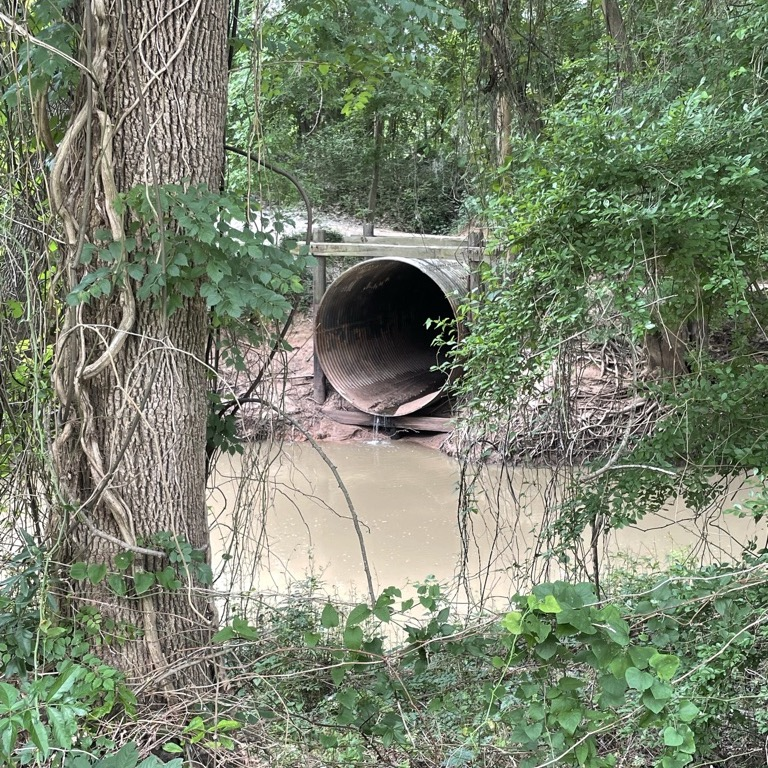
\includegraphics[height=3.5in]{culvert.jpeg}}%
            \hfill
            \subcaptionbox{Bridge Clearance}{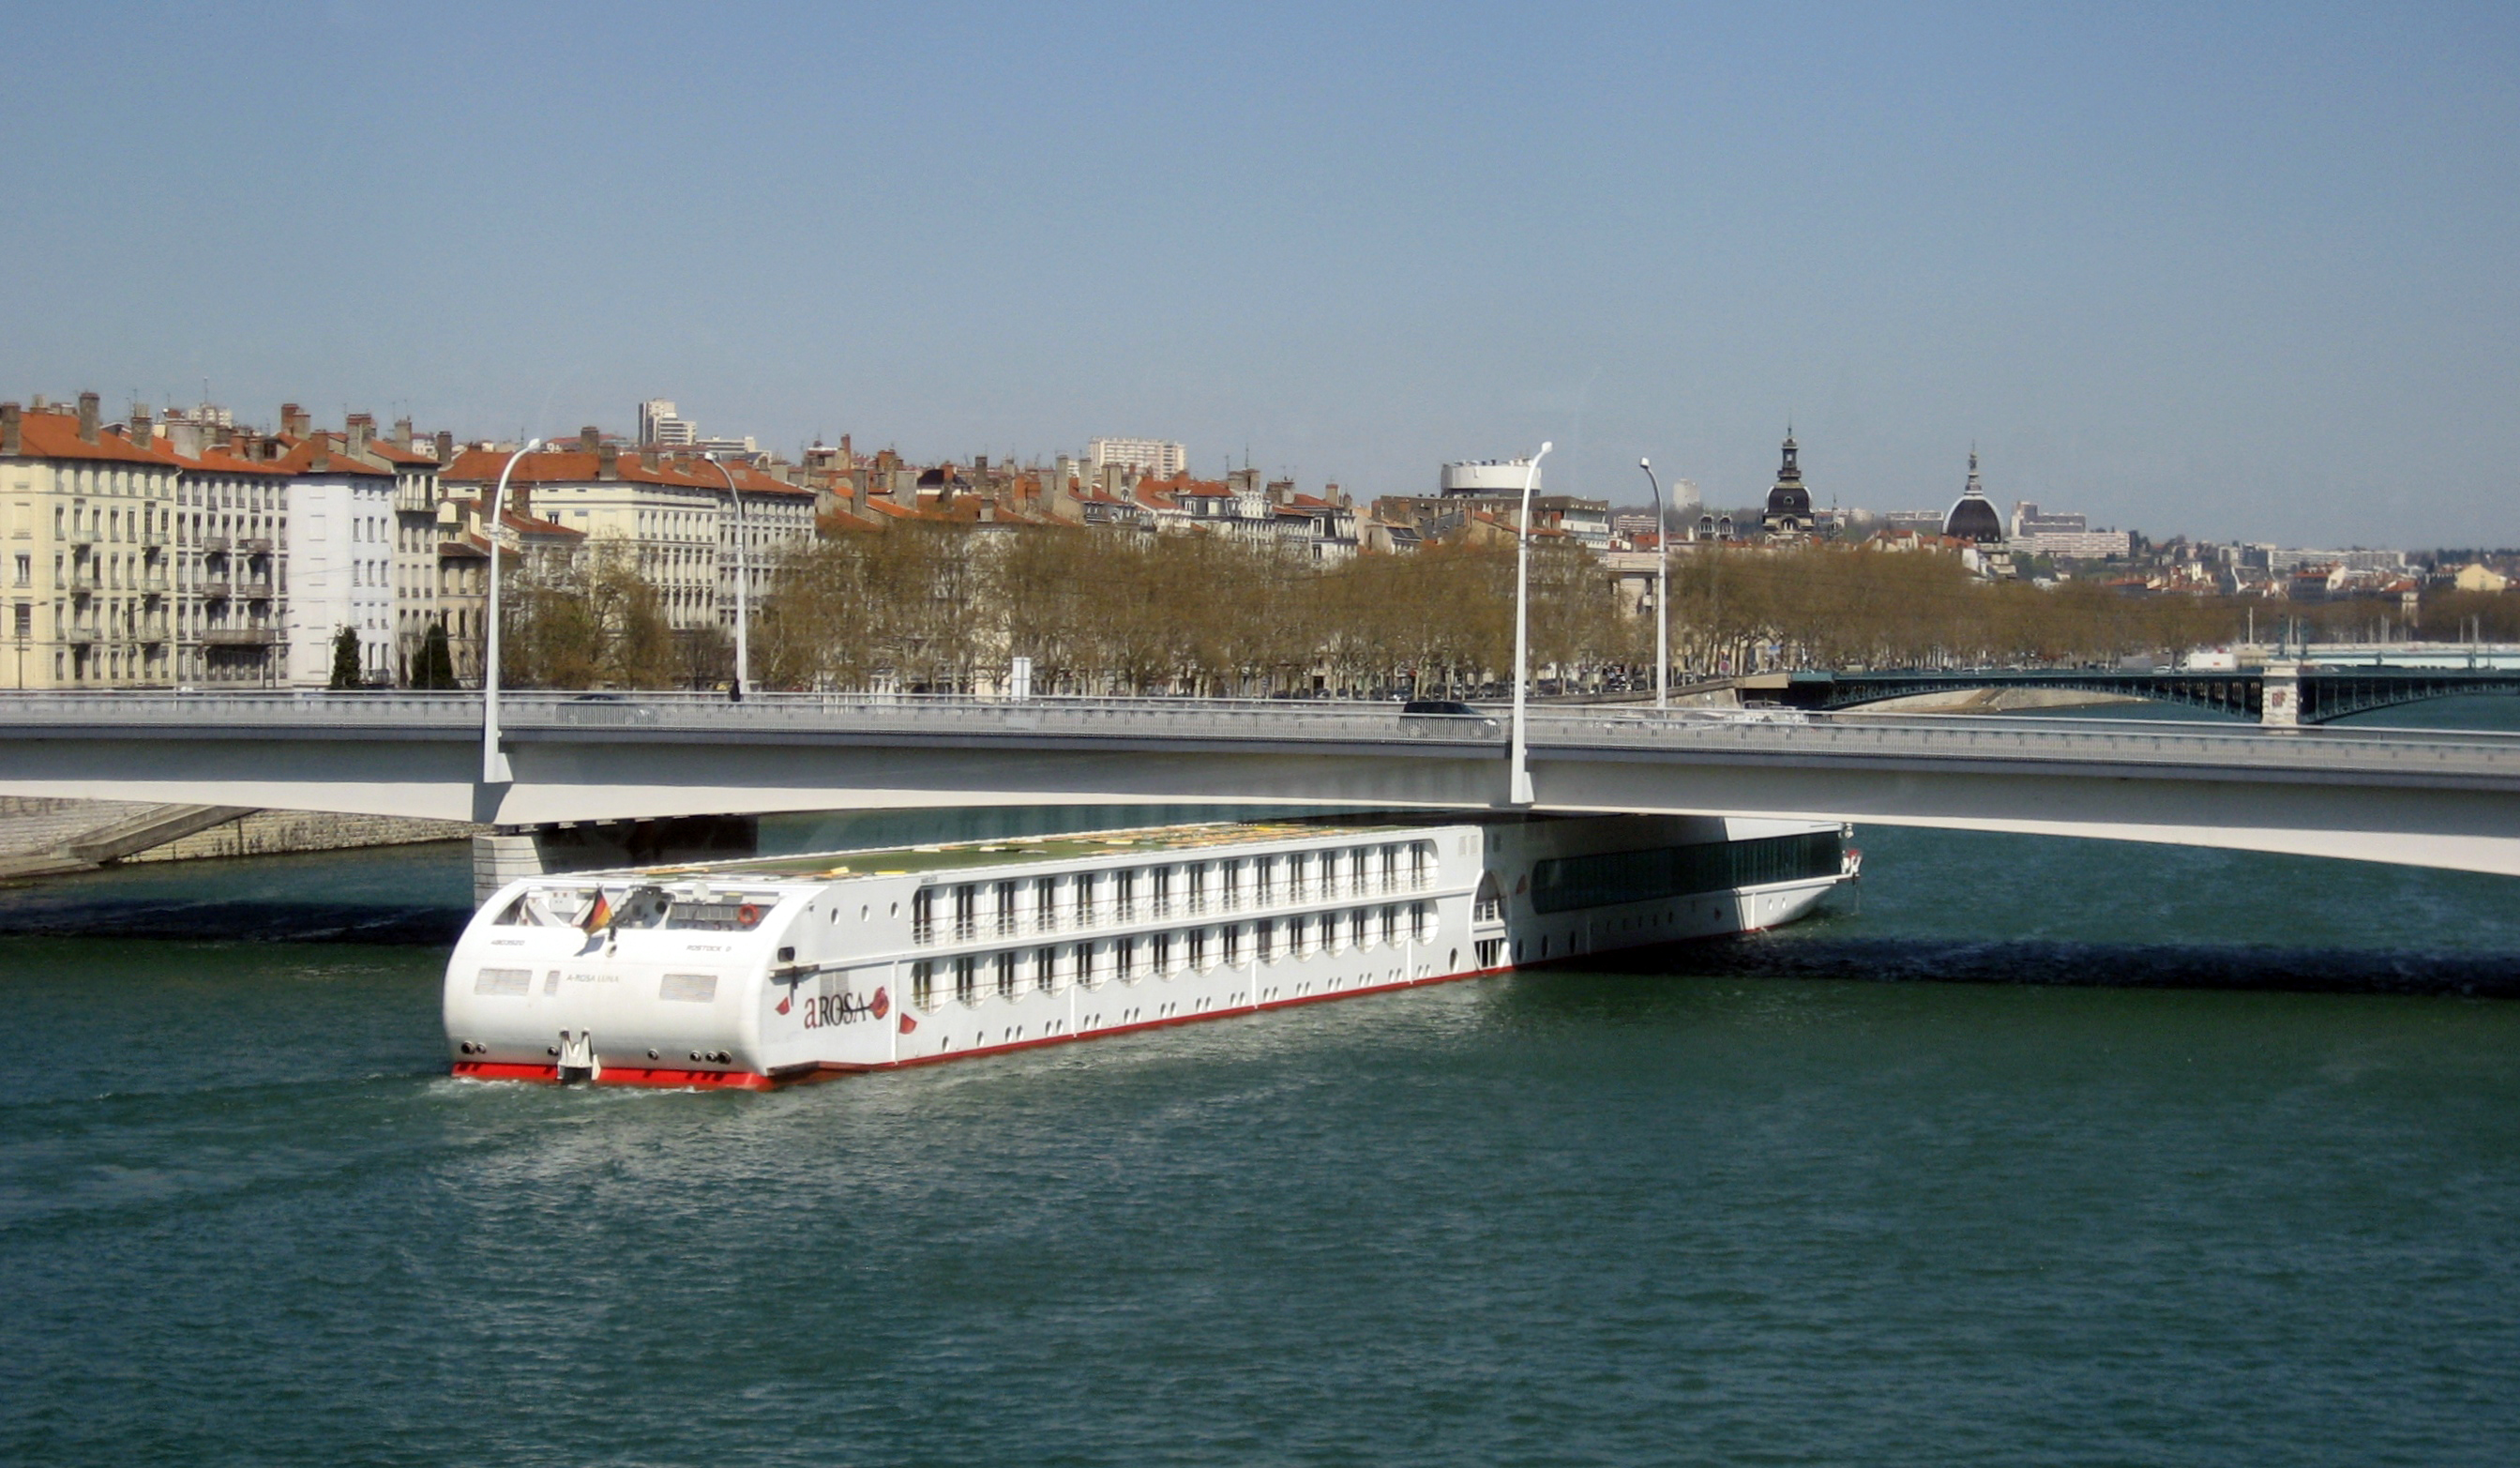
\includegraphics[height=3.5in]{bridge_clearance.jpg}}
            \caption{
                House elevation is just one of many design problems where nonstationary hazards, subject to scenario and model structure uncertainties, drive outcomes.
                \faIcon{camera}: (a) JDG (b) D. Howard / Wikipedia.
            }
            \label{fig:images}
        \end{figure}
    \end{framed}
\end{block}